%导言区
\documentclass{article}

\usepackage{ctex}
\usepackage{graphicx}
 
%标题控制(caption,bicaption等宏包)
%并排与子图表(subcaption,subfig,floatrow等宏包)
%绕排(picinpar,wrapfig等宏包)

%浮动体
%实现灵活分页(避免无法分割的内容产生的页面留白)
%给图表添加标题
%交叉引用

%实现:
%figure环境(table环境与之类似)
%\begin{figure}[<允许位置>]
%	<任意内容>
%\end{figure}

%<允许位置>参数(默认tbp)
%h,此处(here)-代码所在的上下文位置
%t,页顶(top)-代码所在的页面或之后页面的顶部
%b,页底(bottom)-代码所在页面或之后页面的底部
%p,独立一页(page)-浮动页面


%正文区
\begin{document}
	\graphicspath{{figures/}}%设定图片路径
	
	%\ref交叉引用
	\LaTeX{}中\LaTeX 系统的吉祥物-小狮子见图 \ref{fig-lion}
	
	\begin{figure}[htbp] %设置图为浮动体
		\centering			%图片居中
		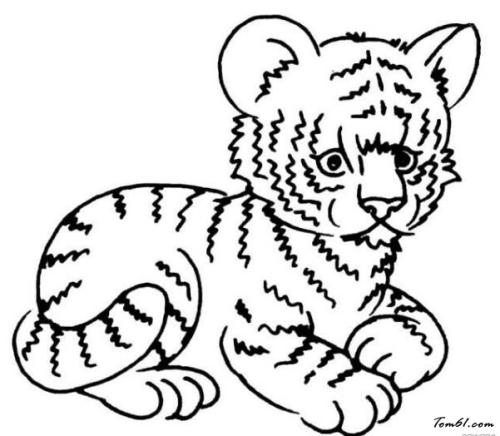
\includegraphics[scale=0.3]{lion}%设定缩放因子
		%为图片添加标题,并设置标签用于交叉引用
		\caption{\LaTeX 系统的吉祥物-小狮子} \label{fig-lion}
	\end{figure}
	
	
	\LaTeX{}中考试成绩,见表格 
	\ref{table-scores}
	
	\begin{table}[htbp]
		\centering
		\caption{考试成绩} 
		\label{table-scores}
		
		\begin{tabular}{|l|| c| c| c| p{2cm}|} %指定列排版格式-左对齐,居中,右对齐
		\hline
		性别 & 语文 & 数学 & 英语 & 备注\\
		\hline \hline
		张三 & 87 & 78 & 87& 优秀\\
		\hline
		李四 & 45 & 56 & 72 & 补考,另行通知\\
		\hline
		王五 & 99 & 56 & 35 & 偏科\\
		\hline
		\end{tabular}
	\end{table}
	
	%\ref交叉引用
	\LaTeX{}中\LaTeX 美丽的乡村-清明上河图见图
	\ref{fig-mountain}
		
	\begin{figure}[htbp] %设置图为浮动体
		\centering			%图片居中
		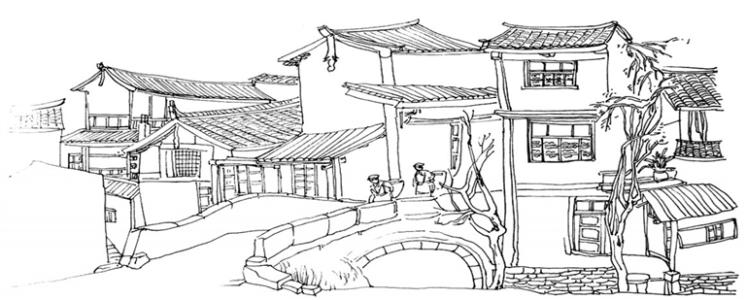
\includegraphics[scale=0.3]{mountain}%设定缩放因子
		%为图片添加标题,并设置标签用于交叉引用
		\caption{\LaTeX 清明上河图} \label{fig-mountain}
	\end{figure}
	
\end{document}